\documentclass[12pt,a4paper,reqno]{amsart}

% language
\usepackage[greek,english]{babel}
\usepackage[utf8]{inputenc}
\usepackage{alphabeta}

% change default names to greek
\addto\captionsenglish{
    \renewcommand{\contentsname}{Περιεχόμενα}
    \renewcommand{\refname}{Βιβλιογραφία}
    \renewcommand{\datename}{Ημερομηνία:}
    \renewcommand{\urladdrname}{Ιστοσελίδα}
}

% math 
\usepackage{amsmath,amsthm,amssymb,amscd}

% font
\usepackage[cal=euler]{mathalfa}
\usepackage{libertinus-type1}
% \usepackage{txfonts} % for upright greek letters
\usepackage{bm} % for bold symbols
\usepackage{bbm} % for the simply-looking bb symbols

% miscellaneous 
\usepackage{changepage} %for indenting environments
\usepackage{csquotes} % example: \textcquote{}
\usepackage{blkarray}
\setcounter{MaxMatrixCols}{20} % default for pmatrix is 10!!
\usepackage{ytableau}
\usepackage{array} %needed to increase the vertical length in a tabular

% drawing
\usepackage{tikz,tikz-cd}
\usetikzlibrary{shapes.misc, patterns, matrix, calc, intersections,positioning}
\usepackage{graphics,graphicx}
\usepackage{float} % provides enhanced control and customization options for floating objects such as figures and tables

% colors
\usepackage{xcolor}
\definecolor{darkcandyapplered}{rgb}{0.64, 0.0, 0.0}
\definecolor{midnightblue}{rgb}{0.1, 0.1, 0.44}
\definecolor{mylightblue}{HTML}{336699}
\definecolor{burntorange}{rgb}{0.8, 0.33, 0.0}
\definecolor{iceberg}{rgb}{0.44, 0.65, 0.82}
\definecolor{applegreen}{rgb}{0.55, 0.71, 0.0}
\definecolor{canaryyellow}{rgb}{1.0, 0.94, 0.0}

% hrefs
\usepackage{hyperref}
\usepackage[noabbrev,capitalize]{cleveref}
\hypersetup{
    pdftoolbar=true,        
    pdfmenubar=true,        
    pdffitwindow=false,     
    pdfstartview={FitH},  % fits the width of the page to the window
    pdftitle={},
    pdfauthor={},
    pdfsubject={},
    pdfkeywords={},
    pdfnewwindow=true,  % links in new window
    colorlinks=true,  % false: boxed links; true: colored links
    linkcolor=darkcandyapplered,   % color of internal links
    citecolor=midnightblue,  % color of links to bibliography
    urlcolor=cyan,  % color of external links
    linktocpage=true  % changes the links from the section body to the page number
    }

% geometry
\textwidth=16cm 
\textheight=21cm 
\hoffset=-55pt 
\footskip=25pt

% thm envs (you might need to change the path)
\theoremstyle{definition}
\newtheorem{theorem}{Θεώρημα}
\newtheorem{proposition}[theorem]{Πρόταση}
\newtheorem{lemma}[theorem]{Λήμμα}
\newtheorem{corollary}[theorem]{Πόρισμα}
\newtheorem{conjecture}[theorem]{Εικασία}
\newtheorem{problem}[theorem]{Πρόβλημα}
\newtheorem*{claim}{Ισχυρισμός}
\newtheorem{observation}[theorem]{Παρατήρηση}
\newtheorem{definition}[theorem]{Ορισμός}
\newtheorem{question}[theorem]{Ερώτημα}
\newtheorem*{questions}{Ερωτήματα}
\newtheorem*{que}{Ερώτημα}
\newtheorem{example}[theorem]{Παράδειγμα}
\newtheorem{exercise}{Άσκηση}

\theoremstyle{remark}
\newtheorem*{remark}{Παρατήρηση}

% fixes the correct numbering of environments
\numberwithin{theorem}{section}
\numberwithin{exercise}{section}
\numberwithin{equation}{section}

% math ops 
% fields
\newcommand{\NN}{\mathbbmss{N}} 
\newcommand{\ZZ}{\mathbbmss{Z}} 
\newcommand{\QQ}{\mathbbmss{Q}} 
\newcommand{\RR}{\mathbbmss{R}} 
\newcommand{\CC}{\mathbbmss{C}} 
\newcommand{\KK}{\mathbbmss{K}} 
\newcommand{\FF}{\mathbbmss{F}} 
\newcommand{\HH}{\mathbbmss{H}} 

% symmetric group
\newcommand{\fS}{\mathfrak{S}}  

% calligraphic 
\newcommand{\aA}{\mathcal{A}} 
\newcommand{\bB}{\mathcal{B}}
\newcommand{\cC}{\mathcal{C}}
\newcommand{\dD}{\mathcal{D}}
\newcommand{\eE}{\mathcal{E}}
\newcommand{\fF}{\mathcal{F}}
\newcommand{\hH}{\mathcal{H}}
\newcommand{\iI}{\mathcal{I}}
\newcommand{\lL}{\mathcal{L}}
\newcommand{\oO}{\mathcal{O}}
\newcommand{\pP}{\mathcal{P}}
\newcommand{\sS}{\mathcal{S}}
\newcommand{\mM}{\mathcal{M}}
\newcommand{\uU}{\mathcal{U}}

% bold
\newcommand{\bfa}{\mathbf{a}}
\newcommand{\bfe}{\mathbf{e}}
\newcommand{\bfF}{\pmb{F}}
\newcommand{\bfR}{\pmb{R}}
\newcommand{\bfv}{\mathbf{v}}
%\newcommand{\bfx}{\bm{x}}
%\newcommand{\bfx}{\mathbf{x}} 
\newcommand{\bfx}{\pmb{x}}
\newcommand{\bfX}{\pmb{X}}
\newcommand{\bfy}{\pmb{y}}
\newcommand{\bfz}{\pmb{z}}

% roman
\newcommand{\rmA}{\mathrm{A}}
\newcommand{\rmB}{\mathrm{B}}
\newcommand{\rmC}{\mathrm{C}}
\newcommand{\rmD}{\mathrm{D}} 
\newcommand{\rmH}{\mathrm{H}} 
\newcommand{\rmh}{\mathrm{h}} 
\newcommand{\rmI}{\mathrm{I}} 
\newcommand{\rmK}{\mathrm{K}}
\newcommand{\rmM}{\mathrm{M}}
\newcommand{\rmP}{\mathrm{P}}  
\newcommand{\rmp}{\mathrm{p}}  
\newcommand{\rmQ}{\mathrm{Q}}  
\newcommand{\rmR}{\mathrm{R}}
\newcommand{\rmS}{\mathrm{S}}
\newcommand{\rmT}{\mathrm{T}}
\newcommand{\rmU}{\mathrm{U}}
\newcommand{\rmV}{\mathrm{V}}
\newcommand{\rmY}{\mathrm{Y}}
\newcommand{\rmZ}{\mathrm{Z}}
\newcommand{\rmz}{\mathrm{z}}

% arrows and symbols 
\renewcommand{\to}{\rightarrow}
\newcommand{\toto}{\longrightarrow}
\newcommand{\mapstoto}{\longmapsto}
\newcommand{\then}{\Rightarrow}
\newcommand{\IFF}{\Leftrightarrow}
\newcommand{\tl}{\tilde}
\newcommand{\wtl}{\widetilde}
\newcommand{\ol}{\overline}
\newcommand{\ul}{\underline}
\newcommand{\oldemptyset}{\emptyset}
\renewcommand{\emptyset}{\varnothing}
\DeclareMathSymbol{\Arg}{\mathbin}{AMSa}{"39} % for arguments 
\newcommand{\onto}{\ensuremath{\twoheadrightarrow}}
\newcommand{\tle}{\trianglelefteq}
\newcommand{\tge}{\trianglerighteq}

% custom ops
\newcommand{\rmKer}{\mathrm{Ker}}
\newcommand{\rmIm}{\mathrm{Im}}
\newcommand{\lcm}{\mathrm{lcm}}
\newcommand{\GL}{\mathrm{GL}}

% absolute value symbol
\usepackage{mathtools} 
\DeclarePairedDelimiter\abs{\lvert}{\rvert}%
\DeclarePairedDelimiter\norm{\lVert}{\rVert}%
\makeatletter
\let\oldabs\abs
\def\abs{\@ifstar{\oldabs}{\oldabs*}}

% tensor symbol
\newcommand{\tensor}[1]{%
  \mathbin{\mathop{\otimes}\limits_{#1}}%
}

% permutation cycle notation
\ExplSyntaxOn
\NewDocumentCommand{\cycle}{ O{\;} m }
 {
  (
  \alec_cycle:nn { #1 } { #2 }
  )
 }

\seq_new:N \l_alec_cycle_seq
\cs_new_protected:Npn \alec_cycle:nn #1 #2
 {
  \seq_set_split:Nnn \l_alec_cycle_seq { , } { #2 }
  \seq_use:Nn \l_alec_cycle_seq { #1 }
 }
\ExplSyntaxOff

% setminus symbol
\newcommand{\mysetminusD}{\hbox{\tikz{\draw[line width=0.6pt,line cap=round] (3pt,0) -- (0,6pt);}}}
\newcommand{\mysetminusT}{\mysetminusD}
\newcommand{\mysetminusS}{\hbox{\tikz{\draw[line width=0.45pt,line cap=round] (2pt,0) -- (0,4pt);}}}
\newcommand{\mysetminusSS}{\hbox{\tikz{\draw[line width=0.4pt,line cap=round] (1.5pt,0) -- (0,3pt);}}}
\newcommand{\sm}{\mathbin{\mathchoice{\mysetminusD}{\mysetminusT}{\mysetminusS}{\mysetminusSS}}}

% miscellaneous commands
\newcommand{\defn}[1]{{\color{mylightblue}{#1}}}
\newcommand{\toDo}{{\bf\color{red} TODO}}
\newcommand{\toCite}{{\bf\color{green} CITE}}
\newcommand*{\vertbar}{\rule[-1ex]{0.5pt}{2.5ex}} % for matrices with column vectors
\newcommand*{\horzbar}{\rule[.5ex]{2.5ex}{0.5pt}} % for matrices with row vectors
\newcommand{\myblue}[1]{{\color{iceberg}{#1}}}
\newcommand{\myorange}[1]{{\color{burntorange}{#1}}}
\newcommand{\mygreen}[1]{{\color{applegreen}{#1}}}
\newcommand{\myred}[1]{{\color{darkcandyapplered}{#1}}}

% ferrer's diagram
\newcommand{\fdiagram}[1]{
    \begin{tikzpicture}[scale=.7]
        \fill foreach \Z [count=\Y] in {#1}
        {foreach \X in {1,...,\Z} 
        {(\X,-\Y) circle[radius=3pt]}};
    \end{tikzpicture}
}

%
\makeatletter
\def\mathcolor#1#{\@mathcolor{#1}}
\def\@mathcolor#1#2#3{%
  \protect\leavevmode
  \begingroup
    \color#1{#2}#3%
  \endgroup
}
\makeatother

% 
\newenvironment{nouppercase}{%
  \let\uppercase\relax%
  \renewcommand{\uppercasenonmath}[1]{}}{}

% titlepage
\title{226: Θεωρία Δακτυλίων και Modules}
\author[Β.~Δ. Μουστακας]{Βασίλης Διονύσης Μουστάκας \\ Πανεπιστήμιο Κρήτης}
\date{19 Φεβρουαρίου 2026}
% \urladdr{\href{https://sites.google.com/view/vasmous}{https://sites.google.com/view/vasmous}}

\begin{document}

\begingroup
\def\uppercasenonmath#1{} % this disables uppercase title
\let\MakeUppercase\relax % this disables uppercase authors
\maketitle
\endgroup

\setcounter{section}{2}
% \setcounter{theorem}{4}
% \setcounter{equation}{}
\begin{center}
    \textbf{2. Δακτύλιοι και παραγοντοποίηση
} 
\end{center}

Τα ιδεώδη του $\ZZ$ που εμφανίστηκαν στην πρώτη ενότητα ήταν όλα κύρια. Αυτό δεν είναι σύμπτωση.
\begin{proposition}
    \label{prop:Z_implies_PID}
    Κάθε ιδεώδες του $\ZZ$ είναι κύριο.
\end{proposition}

\begin{proof}[Απόδειξη]
    Έστω $I$ ένα ιδεώδες του $\ZZ$. Αν $Ι = \{0\} = (0)$, το οποίο είναι κύριο. Διαφορετικά, περιέχει κάποιον θετικό ακέραιο. Έστω $b \in I$ ο μικρότερος τέτοιος. Από τον Ορισμό 1.5 έπεται ότι $(b) \subseteq I$. Αρκεί να δείξουμε ότι $I \subseteq (b)$.

    Έστω $a \in I$. Χωρίς βλάβη της γενικότητας, υποθέτουμε ότι $b \in \NN$. Τότε, υπάρχουν $q, r \in \NN$ τέτοια ώστε 
    \begin{equation}
    \label{eq:euclidean_division}
    a = qb + r
    \end{equation}
    όπου $0 \le r < b$. Όμως,
    \[
    r = \underbrace{\left(r-a\right)}_{\in \ (a) \ \subseteq \ I} + \underbrace{a}_{\in \ I} \ \in \ I
    \]
    όπου η πρώτη σχέση του ανήκει έπεται από την Ταυτότητα \eqref{eq:euclidean_division}. Η επιλογή του $b$ έχει ως αποτέλεσμα $r=0$ και γι αυτό η Ταυτότητα \eqref{eq:euclidean_division} παίρνει την μορφή 
    \[
    a = qb \ \in \ (b)
    \]
    και το ζητούμενο έπεται.
\end{proof}

Το κύριο συστατικό της απόδειξης της Πρότασης \ref{prop:Z_implies_PID} είναι η δυνατότητα να κάνουμε Ευκλείδια διαίρεση στο $\ZZ$.
\begin{definition}
    \label{def:euclidean_domain}
    Έστω $R$ ένας μεταθετικός δακτύλιος. Μια απεικόνιση $N : R \to \NN$ ονομάζεται \defn{Ευκλείδια}\footnote{Μερικές φορές αποκαλείται Ευκλείδια νόρμα ή Ευκλείδια στάθμη.} αν $N(0)=0$ και για κάθε $a, b \in R$ με $b \neq 0$ ισχύει ότι 
    \[
    a = qb + r
    \]
    για κάποια $q, r \in R$ με $r = 0$ ή $N(r) < N(b)$. Ένας μεταθετικός δακτύλιος εφοδιασμένος με μια Ευκλείδια απεικόνιση ονομάζεται \defn{Ευκλείδιος}.
\end{definition}

Οι Ευκλείδιοι δακτύλιοι είναι ακριβώς εκείνοι οι μεταθετικοί δακτύλιοι στους οποίους μπορούμε να κάνουμε Ευκλείδια διαίρεση. Για παράδειγμα, οι $\ZZ$ και $F[x]$ είναι Ευκλείδιοι, όπου $F$ είναι ένα σώμα, με αντίστοιχες Ευκλείδιες απεικονίσεις την απόλυτη τιμή ενός ακεραίου
\[
N(a) = \abs{a}
\]
και τον βαθμό ενός πολυωνύμου
\[
N\left(f(x)\right) = \deg\left(f(x)\right).
\]
Επίσης, κάθε απεικόνιση $N : F \to \NN$ με την ιδιότητα $N(0)=0$ είναι Ευκλείδια (γιατί;). Μπορούμε λοιπόν να φανταστούμε το $N(r)$ σαν ένα μέτρο μεγέθους του στοιχείου $r$.
\begin{example}
    \label{ex:gaussianIntegers_ED}
    Θα δείξουμε ότι ο δακτύλιος των ακεραίων του Gauss 
    \[
    \ZZ[i] = \{x + iy : x, y \in \ZZ\}
    \]
    αποτελεί Ευκλείδια περιοχή με Ευκλείδια απεικόνιση 
    \[
    N(x +iy) = x^2 + y^2.
    \]
    
    Έστω $a, b \in \ZZ[i]$ με $b \neq 0$. Ψάχνουμε $q, r \in \ZZ[i]$ τέτοια ώστε 
    \[
    a = qb + r
    \]
    με $r=0$ ή $N(r) < N(b)$. Παρατηρούμε ότι $N(c) = \abs{c}^2$, για κάθε $c \in \ZZ[i]$, όπου με $\abs{\cdot}$ συμβολίζουμε το μέτρο ενός μιγαδικού αριθμού. Συνεπώς, η συνθήκη $N(r) < N(b)$ είναι ισοδύναμη με 
    \[
    \abs{r}^2 < \abs{b}^2 \ \Leftrightarrow \
    \abs{r} < \abs{b} \ \Leftrightarrow \
    \abs{\frac{r}{b}} = \frac{\abs{r}}{\abs{b}} < 1.
    \]
    Από την άλλη μεριά, η συνθήκη $a = qb + r$ είναι ισοδύναμη με 
    \[
    \frac{a}{b} = q + \frac{r}{b} \ \Leftrightarrow \ \frac{r}{b} = \frac{a}{b} - q.
    \]

    Με άλλα λόγια, συνδυάζοντας αυτές τις παρατηρήσεις, ψάχνουμε ένα $q \in \ZZ[i]$ τέτοιο ώστε 
    \[
    \abs{\frac{a}{b} -q} < 1,
    \]
    δηλαδή θέλουμε τα στοιχεία $a/b$ και $q$ να απέχουν μεταξύ τους απόσταση μικρότερη από $1$ στο μιγαδικό επίπεδο. Σκεπτόμενοι τους ακεραίους του Gauss στο μιγαδικό επίπεδο όπως το πλέγμα $\ZZ\times\ZZ$ στον $\RR^2$ 
    \[
    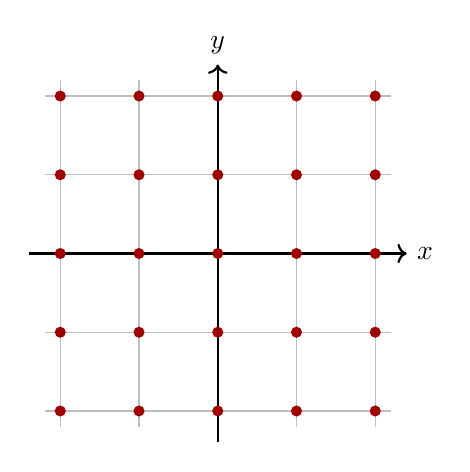
\begin{tikzpicture}[scale=1]
        % Draw grid
        \draw[step=1cm, gray!50, thin] (-2.2,-2.2) grid (2.2,2.2);

        % Highlight axes
        \draw[->, thick] (-2.4,0) -- (2.4,0) node[right] {$x$};
        \draw[->, thick] (0,-2.4) -- (0,2.4) node[above] {$y$};

        % Plot lattice points (Gaussian integers)
        \foreach \x in {-2,-1,0,1,2}
            \foreach \y in {-2,-1,0,1,2}
            \fill[darkcandyapplered] (\x,\y) circle (2pt);
    \end{tikzpicture}
    \]
    αυτό μπορεί πάντα να συμβεί. Πράγματι, χωρίς βλάβη της γενικότητας, ας υποθέσουμε ότι το $a/b$ βρίσκεται στο εξής τετράγωνο
    \[
    \begin{tikzpicture}[scale=2.5]
        % \useasboundingbox(0.8,0.8) rectangle (2.2,2.2);
        \draw[step=1cm,gray,very thin] (0.8,0.8) grid (2.2,2.2);
        \fill[darkcandyapplered](1, 1) circle (1pt) node[below left=2pt]{$\mathcolor{black}{0}$};
        \fill[darkcandyapplered](2, 1) circle (1pt) node[below right=2pt]{$\mathcolor{black}{1}$};
        \fill[darkcandyapplered](1, 2) circle (1pt) node[above left=2pt]{$\mathcolor{black}{i}$};
        \fill[darkcandyapplered](2, 2) circle (1pt) node[above right=2pt]{$\mathcolor{black}{1+i}$};
        % \fill(1.3, 1.6) circle (1pt) node[below left=-2pt]{$a/b$};
        % \draw[iceberg] (1, 1) circle [radius=0.7071];
        % \draw[iceberg] (2, 1) circle [radius=0.7071];
        % \draw[iceberg] (1, 2) circle [radius=0.7071];
        % \draw[iceberg] (2, 2) circle [radius=0.7071];
    \end{tikzpicture}
    \]
    Αν το $a/b$ βρίσκεται στο σύνορο του τετραγώνου, τότε μπορούμε να διαλέξουμε ένα εκ των $0, 1, 1 + i, i \in \ZZ[i]$ και τα δύο σημεία θα απέχουν απόσταση μικρότερη από $1$. Διαφορετικά, αν το $a/b$ βρίσκεται στο εσωτερικό του τετραγώνου
    \[
    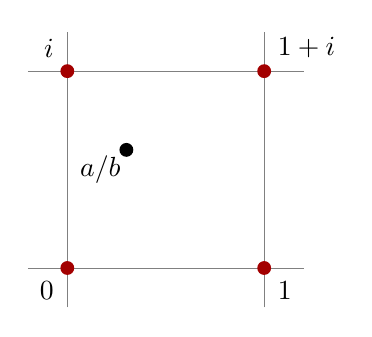
\begin{tikzpicture}[scale=2.5]
        % \useasboundingbox(0.8,0.8) rectangle (2.2,2.2);
        \draw[step=1cm,gray,very thin] (0.8,0.8) grid (2.2,2.2);
        \fill[darkcandyapplered](1, 1) circle (1pt) node[below left=2pt]{$\mathcolor{black}{0}$};
        \fill[darkcandyapplered](2, 1) circle (1pt) node[below right=2pt]{$\mathcolor{black}{1}$};
        \fill[darkcandyapplered](1, 2) circle (1pt) node[above left=2pt]{$\mathcolor{black}{i}$};
        \fill[darkcandyapplered](2, 2) circle (1pt) node[above right=2pt]{$\mathcolor{black}{1+i}$};
        \fill(1.3, 1.6) circle (1pt) node[below left=-2pt]{$a/b$};
        % \draw[iceberg] (1, 1) circle [radius=0.7071];
        % \draw[iceberg] (2, 1) circle [radius=0.7071];
        % \draw[iceberg] (1, 2) circle [radius=0.7071];
        % \draw[iceberg] (2, 2) circle [radius=0.7071];
    \end{tikzpicture}
    \]
    τότε αυτό θα απέχει απέσταση μικρότερη από $\sqrt{2}/2$ (και κατά συνέπεια μικρότερη του $1$) από κάποια από τις κορυφές του τετραγώνου. Πράγματι, θεωρούμε τέσσερις κύκλους με κέντρο τις κορυφές του τετραγώνου και ακτίνα $\sqrt{2}/2$
    \[
    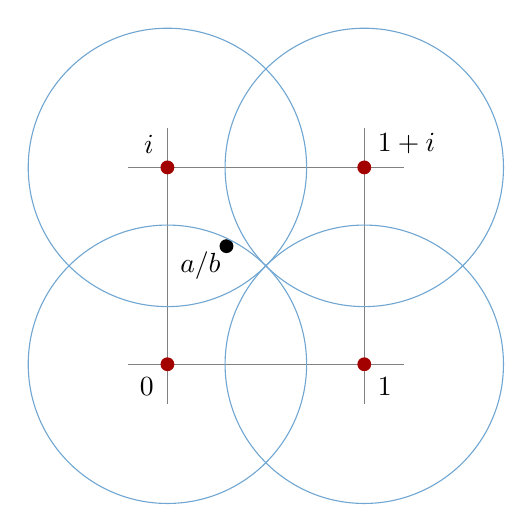
\begin{tikzpicture}[scale=2.5]
        % \useasboundingbox(0.8,0.8) rectangle (2.2,2.2);
        \draw[step=1cm,gray,very thin] (0.8,0.8) grid (2.2,2.2);
        \fill[darkcandyapplered](1, 1) circle (1pt) node[below left=2pt]{$\mathcolor{black}{0}$};
        \fill[darkcandyapplered](2, 1) circle (1pt) node[below right=2pt]{$\mathcolor{black}{1}$};
        \fill[darkcandyapplered](1, 2) circle (1pt) node[above left=2pt]{$\mathcolor{black}{i}$};
        \fill[darkcandyapplered](2, 2) circle (1pt) node[above right=2pt]{$\mathcolor{black}{1+i}$};
        \fill(1.3, 1.6) circle (1pt) node[below left=-2pt]{$a/b$};
        \draw[iceberg] (1, 1) circle [radius=0.7071];
        \draw[iceberg] (2, 1) circle [radius=0.7071];
        \draw[iceberg] (1, 2) circle [radius=0.7071];
        \draw[iceberg] (2, 2) circle [radius=0.7071];
    \end{tikzpicture}
    \]
    Οι κύκλοι αυτοί καλύπτουν όλο το τετράγωνο και το ζητούμενο έπεται.
\end{example}

\begin{proposition}
    \label{prop:ED_implies_PID}
    Σε έναν Ευκλείδιο δακτύλιο κάθε ιδεώδες είναι κύριο.
\end{proposition}

Η απόδειξη της Πρότασης \ref{prop:ED_implies_PID} είναι ίδια με αυτή της Πρότασης \ref{prop:Z_implies_PID} με τη διαφορά ότι σε αυτή την περίπτωση διαλέγουμε το $b$ να είναι τέτοιο ώστε η $N(b)$ να έχει την μικρότερη δυνατή τιμή μεταξύ των στοιχείων του $I$.

Το αντίστροφο της Πρότασης \ref{prop:ED_implies_PID} όμως δεν ισχύει. Ένα αντιπαράδειγμα αποτελεί ο δακτύλιος $\ZZ[\omega] \coloneqq \{x +\omega{y} : x, y \in \ZZ\}$, όπου 
\[
\omega = \frac{1 + \sqrt{-19}}{2}
\]
(βλ. παράδειγμα στην σελίδα 282 του \cite{DF04}).

\begin{definition}
    \label{def:PID}
    Μια ακέραια περιοχή της οποίας κάθε ιδεώδες είναι κύριο ονομάζεται \defn{περιοχή κύριων ιδεωδών} (\defn{ΠΚΙ}) (principal ideal domain (PID)).
\end{definition}

Οι Προτάσεις \ref{prop:Z_implies_PID}και \ref{prop:ED_implies_PID} μας πληροφορούν ότι ο δακτύλιος των ακεραίων και γενικότερα κάθε Ευκλείδια περιοχή είναι περιοχές κύριων ιδεωδών. Μέχρι στιγμής έχουμε συναντήσει τις εξής έννοιες
\begin{table}[H]
\centering
\renewcommand{\arraystretch}{1.3} 
\begin{tabular}{c|l}
\textbf{δακτύλιος}     & \textbf{ιδιότητα του $\ZZ$ που γενικεύει} \\ \hline
ακέραια περιοχή        & το γινόμενο δύο μη μηδενικών στοιχείων είναι μη μηδενικό \\ \hline
Ευκλείδια περιοχή      & Ευκλείδια διαίρεση \\ \hline
Περιοχή κύριων ιδεωδών & κάθε ιδεώδες είναι κύριο 
\end{tabular}
\end{table}
\noindent
στην μελέτη της αριθμητικής των δακτυλίων, οι οποίες γενικεύουν την αντίστοιχη ιδιότητα του δακτύλιου των ακεραίων. Το \emph{θεμελιώδες θεώρημα της αριθμητικής} μας πληροφορεί την μονοσήμαντη παραγοντοποίηση ενός ακεραίου σε πρώτους αριθμούς. Ποιά θα ήταν η αντίστοιχη ιδιότητα για έναν αυθαίρετο δακτύλιο; Ποιά είναι η ιδιότητα των πρώτων αριθμών που κάνει την απόδειξη να λειτουργεί; Ως προς τι είναι μοναδική αυτή η παραγοντοποίηση;

\begin{definition}
    \label{def:unit}
    Έστω $R$ ένας δακτύλιος και $u \in R$ ένα μη μηδενικό στοιχείο. Το $u$ ονομάζεται \defn{αντιστρέψιμο} (unit) αν 
    \[
    ur = ru = 1
    \]
    για κάποιο $r \in R$.
\end{definition}

Για παράδειγμα, τα αντιστρέψιμα στοιχεία του $\ZZ$ είναι τα $\pm1$ (γιατί;). Τα αντιστρέψιμα στοιχεία του δακτύλιου των πινάκων $\rmM_n(\RR)$ είναι ακριβώς οι αντιστρέψιμοι πίνακες που συναντήσαμε στη Γραμμική Άλγεβρα, δηλαδή 
\[
{\rmM_n(\RR)}^\times = \GL_n(\RR) \coloneqq \{A \in \rmM_n(\RR) : \det(A) \neq 0\}.
\]
Τι κοινό έχουν αυτά τα δύο σύνολα;

Το σύνολο $R^\times$ όλων των αντιστρέψιμων στοιχείων ενός δακτύλιου $R$ αποτελεί ομάδα ως προς τον πολλαπλασιασμό με ουδέτερο στοιχείο το $1$. Οι δακτύλιοι με τα περισσότερα αντιστρέψιμα στοιχεία είναι τα σώματα $F$. Το $F^\times = F \sm \{0\}$ συχνά αποκαλείται η πολλαπλαστική ομάδα του $F$.

\begin{remark}
    Υποθέτουμε ότι ο $R$ είναι μεταθετικός και έστω $u \in R^\times$. Από τον Ορισμό \ref{def:unit} έπεται ότι $1 \in (u)$ και γι αυτό $(1) \subseteq (u)$. Συνεπώς $(u) = R$. Με άλλα λόγια, τα αντιστρέψιμα στοιχεία σε έναν (μεταθετικό) δακτύλιο συμπεριφέρονται σαν μονάδες υπό αυτή την έννοια. Αυτό εξηγεί την αγγλική ορολογία unit.
\end{remark}

\begin{definition}
    \label{def:irreducible_prime}
    Έστω $R$ ένας μεταθετικός δακτύλιος. Ένα μη μηδενικό, μη αντιστρέψιμο $r \in R$ ονομάζεται 
    \begin{itemize}
        \item \defn{ανάγωγο} (irreducible) στο $R$ αν 
        \[
        r = ab \quad \then \quad a \in R^\times \ \ \text{ή} \ \ b \in R^\times.
        \]
        \item \defn{πρώτο} (prime) στο $R$ αν 
        \[
        r \mid (ab) \quad \then \quad r \mid (a) \ \ \text{ή} \ \ r \mid (b),
        \]
    \end{itemize}
    όπου γράφουμε $r \mid x$ αντί για $x \in (r)$.
\end{definition}

Σκεπτόμενοι τα αντίστροφα στοιχεία ως εκείνα τα στοιχεία που \textquote{συμπεριφέρονται} ως μονάδες με την έννοια της παρατήρησης, τότε τα ανάγωγα στοιχεία ενός δακτύλιου μπο\-ρούμε να τα φανταστούμε ως \emph{δομικά συστατικά} ενός αυθαίρετου στοιχείου ως προς τον πολλαπλασιασμό. Στην περίπτωση όπου $R = \ZZ$ οι έννοιες ανάγωγο και πρώτο στοιχείο ταυτίζονται (γιατί;). Παρακάτω θα δούμε ότι το ίδιο ισχύει σε κάθε περιοχή κύριων ιδεωδών. Συνεπώς, τα δομικά συστατικά σε μια περιοχή κύριων ιδεωδών συμπεριφέρονται ακριβώς όπως και οι πρώτοι αριθμοί στο $\ZZ$. Γενικότερα, ισχύει το εξής.
\begin{proposition}
    \label{prop:prime_implies_irreducible}
    Σε μία ακέραια περιοχή, κάθε πρώτο στοιχείο είναι ανάγωγο.
\end{proposition}
\begin{proof}[Απόδειξη]
    Έστω $R$ μια ακέραια περιοχή και $p \in R$ ένα πρώτο στοιχείο τέτοιο ώστε $p = ab$, για κάποια $a, b \in R$. Επειδή το $p$ είναι πρώτο έπεται ότι $p \mid a$ ή $p \mid b$. Στην πρώτη περίπτωση έχουμε $a = rp$ για κάποιο $r \in R$ και γι αυτό 
    \[
    p = ab = rpb \ \Leftrightarrow \ p(1-rb) = 0.
    \]
    Επειδή ο $R$ είναι ακέραια περιοχή\footnote{Ισοδύναμα, θα μπορούσαμε να \textquote{διαγράψουμε} το $p$ στην εξίσωση $p = p(rb)$ γιατί ο $R$ δεν έχει μηδενοδιαιρέτες. Αυτό ονομάζεται \emph{νόμος διαγραφής}.} και $p \neq 0$ έπεται ότι 
    \[
    1 - rb = 0 \ \then \ rb = 1
    \]
    και γι αυτό $b \in R^\times$. Ομοίως, στην δεύτερη περίπτωση προκύπτει ότι $a \in R^\times$.
\end{proof}

\begin{example}
    \label{ex:irreducible_not_prime}
    Το αντίστροφο της Πρότασης \ref{prop:prime_implies_irreducible} δεν ισχύει. Στο δακτύλιο $R = \ZZ[\sqrt{-3}]$, όπου 
    \[
    \ZZ[\sqrt{-3}] \coloneqq \{x + y\sqrt{-3} : x, y \in \ZZ\}
    \]
    έχουμε 
    \[
    4 \ = \ 2 \cdot 2 \ = \ (1 + \sqrt{-3})(1 - \sqrt{-3}).
    \]
    Συνεπώς, το $2$ δεν μπορεί να είναι πρώτο (γιατί;). Θα δείξουμε ότι είναι ανάγωγο στον $R$.

    Για τον λόγο αυτό, πρώτα θα υπολογίσουμε το $R^\times$. Θεωρούμε την απεικόνιση $\delta : R \to \NN$ που ορίζεται θέτοντας 
    \[
    \delta(x + y\sqrt{-3}) = x^2 + 3y^2.
    \]
    Η απεικόνιση $\delta$ είναι \emph{πολλαπλαστική}, δηλαδή 
    \[
    \delta(ab) = \delta(a)\delta(b)
    \]
    (γιατί;). Ισχυριζόμαστε ότι 
    \[
    R^\times = \{a \in R : \delta(a) = 1\}.
    \]

    Πράγματι, αν $a \in R^\times$, τότε $ab =1$ για κάποιο $b \in R$ και γι αυτό $1 = \delta(a)\delta(b)$ που έχει ως συνέπεια $\delta(a) = 1$ (γιατί;). Αντιστρόφως, αν $a = x + y\sqrt{-3} \in R$ είναι τέτοιο ώστε $\delta(a) = 1$, τότε 
    \[
    a(x - y\sqrt{-3}) = (x + y\sqrt{-3})(x - y\sqrt{-3}) = x^2 + 3y^2 = \delta(a) = 1
    \]
    και γι αυτό $a \in R^\times$.

    Με άλλα λόγια, τα αντιστρέψιμα στοιχεία $a = x + y\sqrt{-3}$ χαρακτηρίζονται από την συνθήκη 
    \[
    x^2 + 3y^2 = 1
    \]
    για $x, y \in \ZZ$. Όμως, οι μόνες λύσεις αυτής της διοφαντικής εξίσωσης είναι $(\pm1,0)$ (γιατί;). Κατά συνέπεια\footnote{Το ίδιο επιχείρημα λειτουργεί αν αντικαταστήσουμε το $3$ με οποιονδήποτε θετικό ακέραιο $d$. Αυτό συμφωνεί με τη διαίσθησή μας, καθώς ο δακτύλιος $\ZZ[\sqrt{-d}]$ ουσιαστικά επεκτείνει τον $\ZZ$ (του οποίου τα αντιστρέψιμα στοιχεία είναι $\pm1$) με την ελάχιστη δυνατή έξτρα δομή, δηλαδή \textquote{επισυνάπτοντας} την λύση της εξίσωσης $x^2 + d = 0$.},
    \[
    R^\times = \{\pm1\}.
    \]

    Ας δείξουμε τώρα ότι το $2$ είναι ανάγωγο στον $R$. Αν $2 = ab$ για κάποια $a, b \in R$, τότε $4 = \delta(a)\delta(b)$ και γι αυτό έχουμε τρεις περιπτώσεις
    \[
    \renewcommand{\arraystretch}{1.3} 
    \begin{tabular}{c|c|c|c}
    $\delta(a)$ & $1$ & $4$ & $2$\\ \hline
    $\delta(b)$ & $4$ & $1$ & $2$
    \end{tabular}
    \]
    Στις πρώτες δύο περιπτώσεις έπεται ότι $a \in R^\times$ και $b \in R^\times$, αντίστοιχα, από τον υπολογισμό που μόλις κάναμε. Η τρίτη περίπτωση είναι αδύνατη (γιατί;).
\end{example}

Πίσω στην αναλογία με το θεμελιώδες θεώρημα της αριθμητικής, στο $\ZZ$ έχουμε τις εξείς παραγοντοποιήσεις 
\[
6 = 2 \cdot 3 = 3 \cdot 2 = (-2)\cdot(-3) = (-3)\cdot(-2).
\]
Τα στοιχεία $\pm2, \pm3$ είναι ανάγωγα στο $\ZZ$ (γιατί;). Υπό ποιά έννοια είναι αυτή η παραγοντο\-ποίηση μοναδική;
\begin{definition}
    \label{def:associate}
    Έστω $R$ ένας μεταθετικός δακτύλιος. Δύο (μη μηδενικά) στοιχεία $a, b \in R$ ονομάζονται \defn{συντροφικά} (associates) αν 
    \[
    a = ub,
    \]
    για κάποιο $u \in R^\times$.
\end{definition}

Με άλλα λόγια, δυο στοιχεία είναι συντροφικά αν διαφέρουν κατά πολλαπλασιασμό με ένα αντίστροφο στοιχείο. Είναι εύκολο να παρατηρήσει κανείς ότι τα $a, b$ είναι συντροφικά αν και μόνο αν $(a) = (b)$ ή ισοδύναμα αν $a \mid b$ και $b \mid a$. Για περισσότερες πληροφορίες, παραπέμπουμε στο \cite[Ενότητα 11.2]{Mpe15}. 

\begin{definition}
    \label{def:UFD}
    Μια ακέραια περιοχή $R$ ονομάζεται\footnote{Κάποιες φορές αναφέρεται και ως περιοχή μοναδικής/μονοσήμαντης ανάλυσης.} \defn{περιοχή μονοσήμαντης παραγοντο\-ποίησης} (\defn{ΠΜΠ}) (unique factorization domain (UFD)) αν κάθε μη μηδενικό, μη αντιστρέψιμο $r \in R$
    \begin{itemize}
        \item[(1)] μπορεί να γραφεί ως γινόμενο πεπερασμένου πλήθους ανάγωγων στοιχείων του $R$
        \item[(2)] η παραγοντοποίηση αυτή είναι μοναδική ως προς αναδιατάξεις των μερών της και ως προς συντροφικότητα, δηλαδή αν 
        \[
        r \ = \ p_1p_2\cdots p_n \ = \ q_1q_2 \cdots q_m 
        \]
        για κάποια ανάγωγα στοιχεία $p_1, p_2, \dots, p_n, q_1, q_2, \dots, q_m \in R$, τότε $n = m$ και 
        \[
        q_{\pi(i)} = u_ip_i
        \]
        για κάθε $1 \le i \le n$, για κάποια μετάθεση\footnote{\emph{Μετάθεση} ενός πεπερασμένου συνόλου $X$ ονομάζεται μια 1-1 και επί απεικόνιση $X \to X$. Το σύνολο των μεταθέσεων συμβολίζεται με $\rmS(X)$. Αν $X = \{1, 2, \dots, n\}$, τότε γράφουμε $\rmS_n$ αντί για $\rmS(X)$. Το σύνολο $\rmS_n$ αποτελεί ομάδα ως προς τη σύνθεση μεταθέσεων και ονομάζεται \emph{συμμετρική ομάδα βαθμού $n$}. Για περισσότερες πληοροφορίες, παραπέμπουμε στο \cite[Ενότητα~1.3]{DF04}} $\pi \in \rmS_n$ και κάποια $u_1, u_2, \dots, u_n \in R^\times$.
    \end{itemize}
\end{definition}

To θεμελιώδες θεώρημα της αριθμητικής και το γεγονός ότι $\ZZ^\times = \{\pm1\}$ μας πληοροφούν ότι ο δακτύλιος των ακεραίων είναι περιοχή μονοσήμαντης παραγοντοποίησης. Από την άλλη μεριά, ο δακτύλιος $\ZZ[\sqrt{-3}]$ δεν είναι περιοχή μονοσήμαντης παραγοντοποίησης, διότι 
\[
    4 \ = \ 2 \cdot 2 \ = \ (1 + \sqrt{-3})(1 - \sqrt{-3})
\]
και οι παράγοντες $2, 1 \pm \sqrt{-3}$ είναι ανάγωγοι (βλ. Παράδειγμα \ref{ex:irreducible_not_prime}), αλλά όχι συντροφικοί (γιατί;).


\begin{thebibliography}{99}
    \bibitem{Mpe15}
    Α. Μπελιγιάννης, 
    \textit{Μια Εισαγωγή στη Βασική Άλγεβρα},
    Κάλλιπος, 2015. (διαθέσιμο \href{https://dx.doi.org/10.57713/kallipos-547}{εδώ})
    %
    \bibitem{DF04}
    D. S. Dummit και R. M. Foote, 
    \textit{Abstract algebra},
    third edition, Wiley, 2004. 
\end{thebibliography}
\end{document}